\subsection{Stiff problem with adaptive step size II}

As next problem we consider the the Statospheric reaction Problem form \cite{sandu2001positive}.
This Modell describes atmospheric Reaction between the substances in the concentration vector $u=[O^{1D},O,O_3,O_2,'NO,NO_2]$. 
The Problem is time dependent and has two linear invariants.

The problem describes as follows:
\begin{align}
    T &= ((t/3600)+t_start) \bmod 24 
    \qquad  Tr = 4.5
    \qquad  Ts = 19.5 \\
    \sigma(T) &= 
     \begin{cases}
    0.5+0.5 \cos(\pi\left|\frac{(2T-Tr-Ts)}{(Ts-Tr)}\right| \left[\frac{(2T-Tr-Ts)}{(Ts-Tr)}\right]       & \quad \text{if } Tr \leq T \leq Ts\\
    0  & \quad \text{else } 
    \end{cases}
\end{align}


\begin{align}
r_1 &= O_2\,k_1       &  k_1 &= \num{2.643e-10} \sigma^3 \\
r_2 &= O\,O_2 k_2     &  k_2 &= \num{8.018e-17} \\
r_3 &= O_3\,k_3       &  k_3 &= \num{6.120e-4}\sigma \\
r_4 &= O_3\,O\,k_4     &  k_4 &= \num{1.567e-15} \\
r_5 &= O_3\,k_5       &  k_5 &= \num{1.070e-3}\sigma^2 \\
r_6&= O^{1D}\,M\,k_6     &  k_6 &= \num{7.110e-11} \\
r_7 &= O^{1D}\,O_3\,k_7   &  k_7 &= \num{1.200e-10} \\
r_8 &= O_3\,NO\,k_8    &  k_8 &= \num{6.062e-15} \\
r_9 &= NO_2\,O\,k_9    &  k_9 &= \num{1.069e-11} \\
r_{10}&=NO_2\,k_{10}  &  k_{10}&=\num{1.289e-2}\sigma \\
r_{11}&=NO\,O\,k_{11} &  k_{11}&=\num{1.0e-8}
\end{align}  

with $M  = 8.120e16$ 

\begin{align}
\frac{\mathrm d}{\mathrm d t}O^{1D}  &=   +r_5 -r_6 -  r_7 \\
\frac{\mathrm d}{\mathrm d t}dO   &=  +2*r_1 -r_2 +r_3 -  r_4  +r_6 -r_9 +r_{10} -r_{11} \\
\frac{\mathrm d}{\mathrm d t}dO_3  &=  +r_2 -r_3 -  r_4 -r_5  -r_7 -r_8 \\
\frac{\mathrm d}{\mathrm d t}dO_2  &=  -r_1 -r_2 +r_3 +2r_4 +r_5 +2r_7 +r_8 +r_9 \\
\frac{\mathrm d}{\mathrm d t}dNO  &=  -r_8 +r_9 +r_{10} -r_{11} \\
\frac{\mathrm d}{\mathrm d t}dNO_2 &=  +r_8 -r_9 -r_{10} +r_{11} 
\end{align}

The two linear invariants are 
\begin{align}
m_O = [1,1,3,2,1,2]^T & \qquad m_O^Tu=\text{const} \\
m_N = [0,0,0,0,1,1]^T & \qquad m_N^Tu=\text{const}
\end{align}

The initial conditions are $u(0)=[\num{9.906e+1},\num{6.624e08},\num{5.326e11},\num{1.697e16},\num{4.000e6},\num{1.093e9}]$
The system was normalized internally such that $u_n(0)=1$ to achieve an suitable error estimation. After the computation the results are scaled back.
The system is solved in the time from $t_{start}=12h$ to $t_{end}=84h$. Using the adapted implicit is done using the Im-Euler~3 extrapolation method with free adaptation. 
Also the same step size control is used. 
The results are plotted in figure\,\ref{fig:Stratospheric_time}. We can see that the results of the adapted solution is close to the reference solution obtained with the unadapted Im-Euler~3 extrapolation method and a higher accuracy.

\begin{figure}
\centering
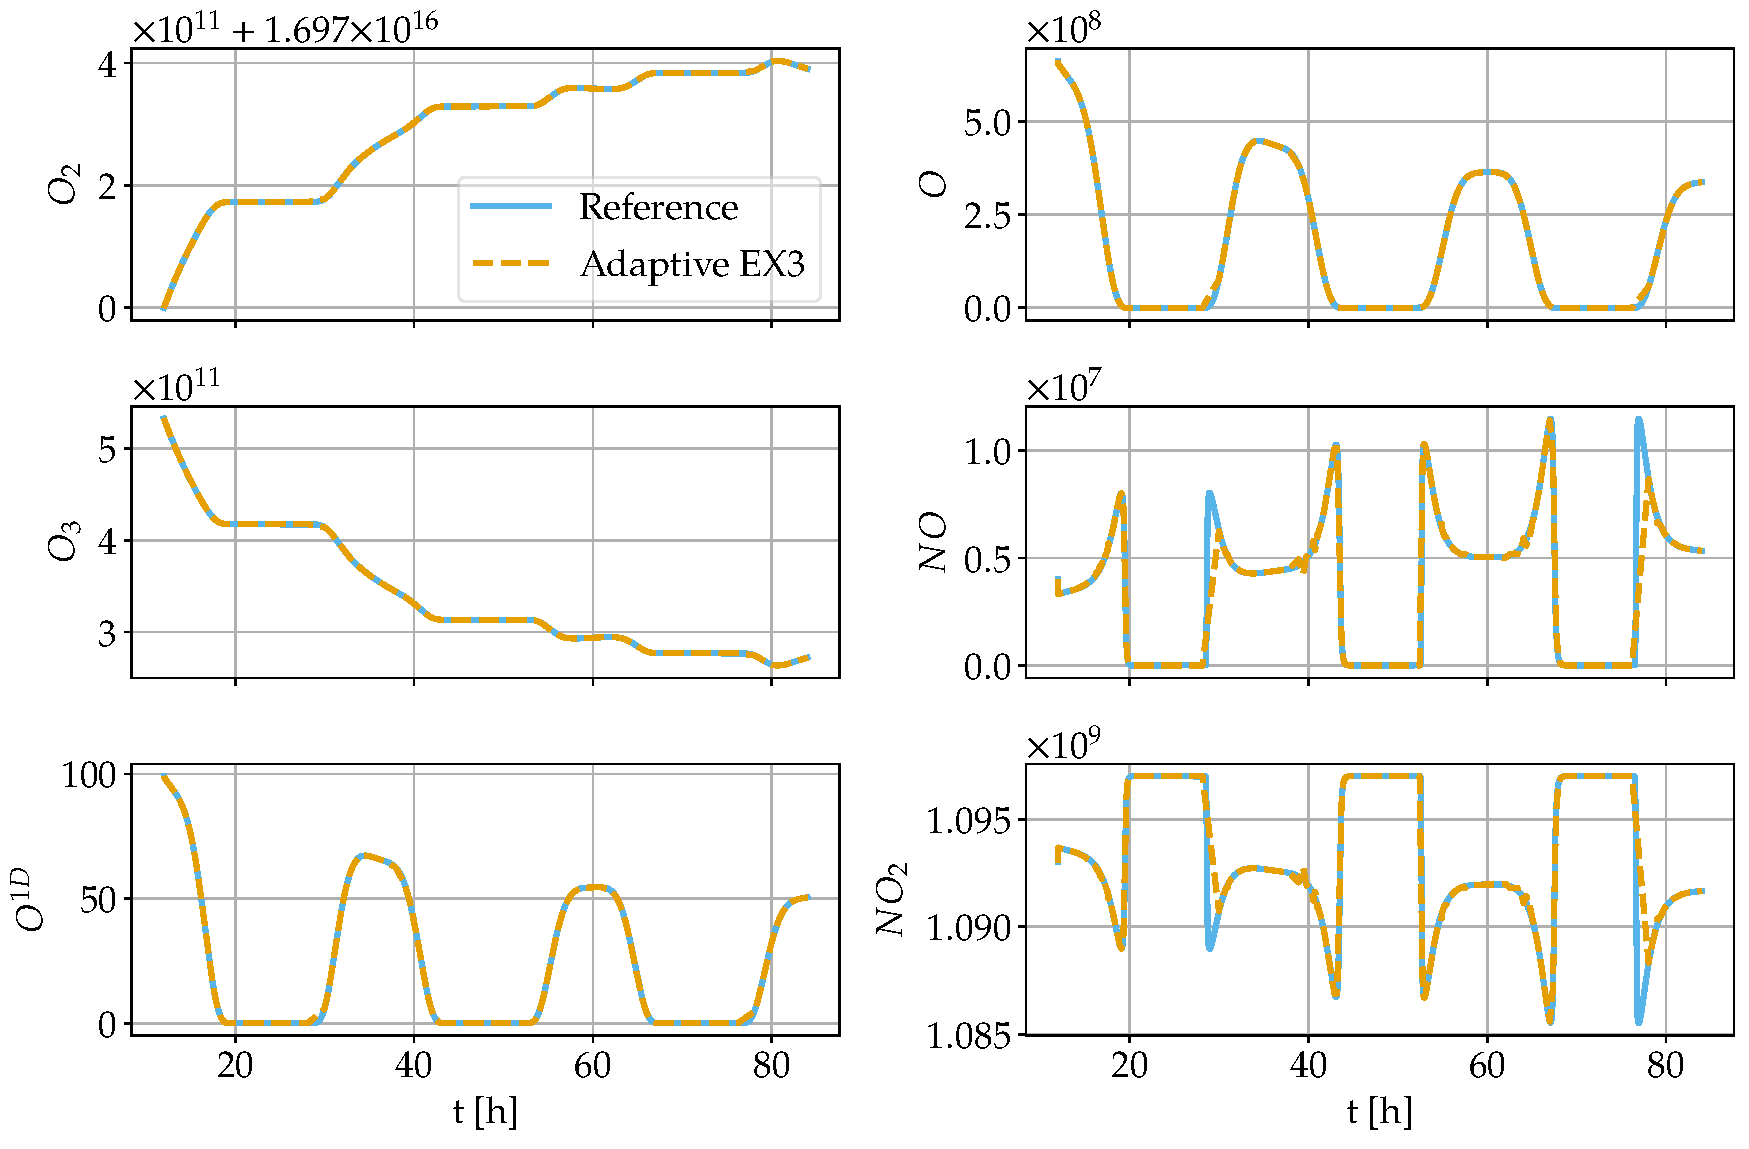
\includegraphics[width=0.9\textwidth]{plots/Stratospheric_time.pdf}
\caption{Numerical approximation of stratospheric reaction system. A reference solution is also plotted}
\label{fig:Stratospheric_time}
\end{figure}

To compute the solution 249 steps were computed, two of these were rejected due to a violation of the error bound.
More details are plotted in figure\,\ref{fig:Stats_Strat}. The rejected steps are drawn with thick crosses.
In the first subplot it can be seen that the step size undergoes multiple sudden changes due to the timedependence of the problem.
The minimum values before and after the adaptation are also drawn for all steps where the initial values where negative. 
This was only the case for some time intervals. 25 Steps exhibited negative values.
Almost all of them very close to 0 and the adaptation did only show a small improvement. 
The smallest value of the solution is $min(u) = \num{-1.59e-11}$.
The used weights are also very close to the original weights, except of the steps that were rejected anyway due to an violation of the tolerance.
The change of the two linear invariantes are plotted in the last two subplots. Both are preserved within roundoff error.
Due to the internal normalization the round off error is amplified to the order of $10$ for $m_O^Tu$. 



\begin{figure}
\centering
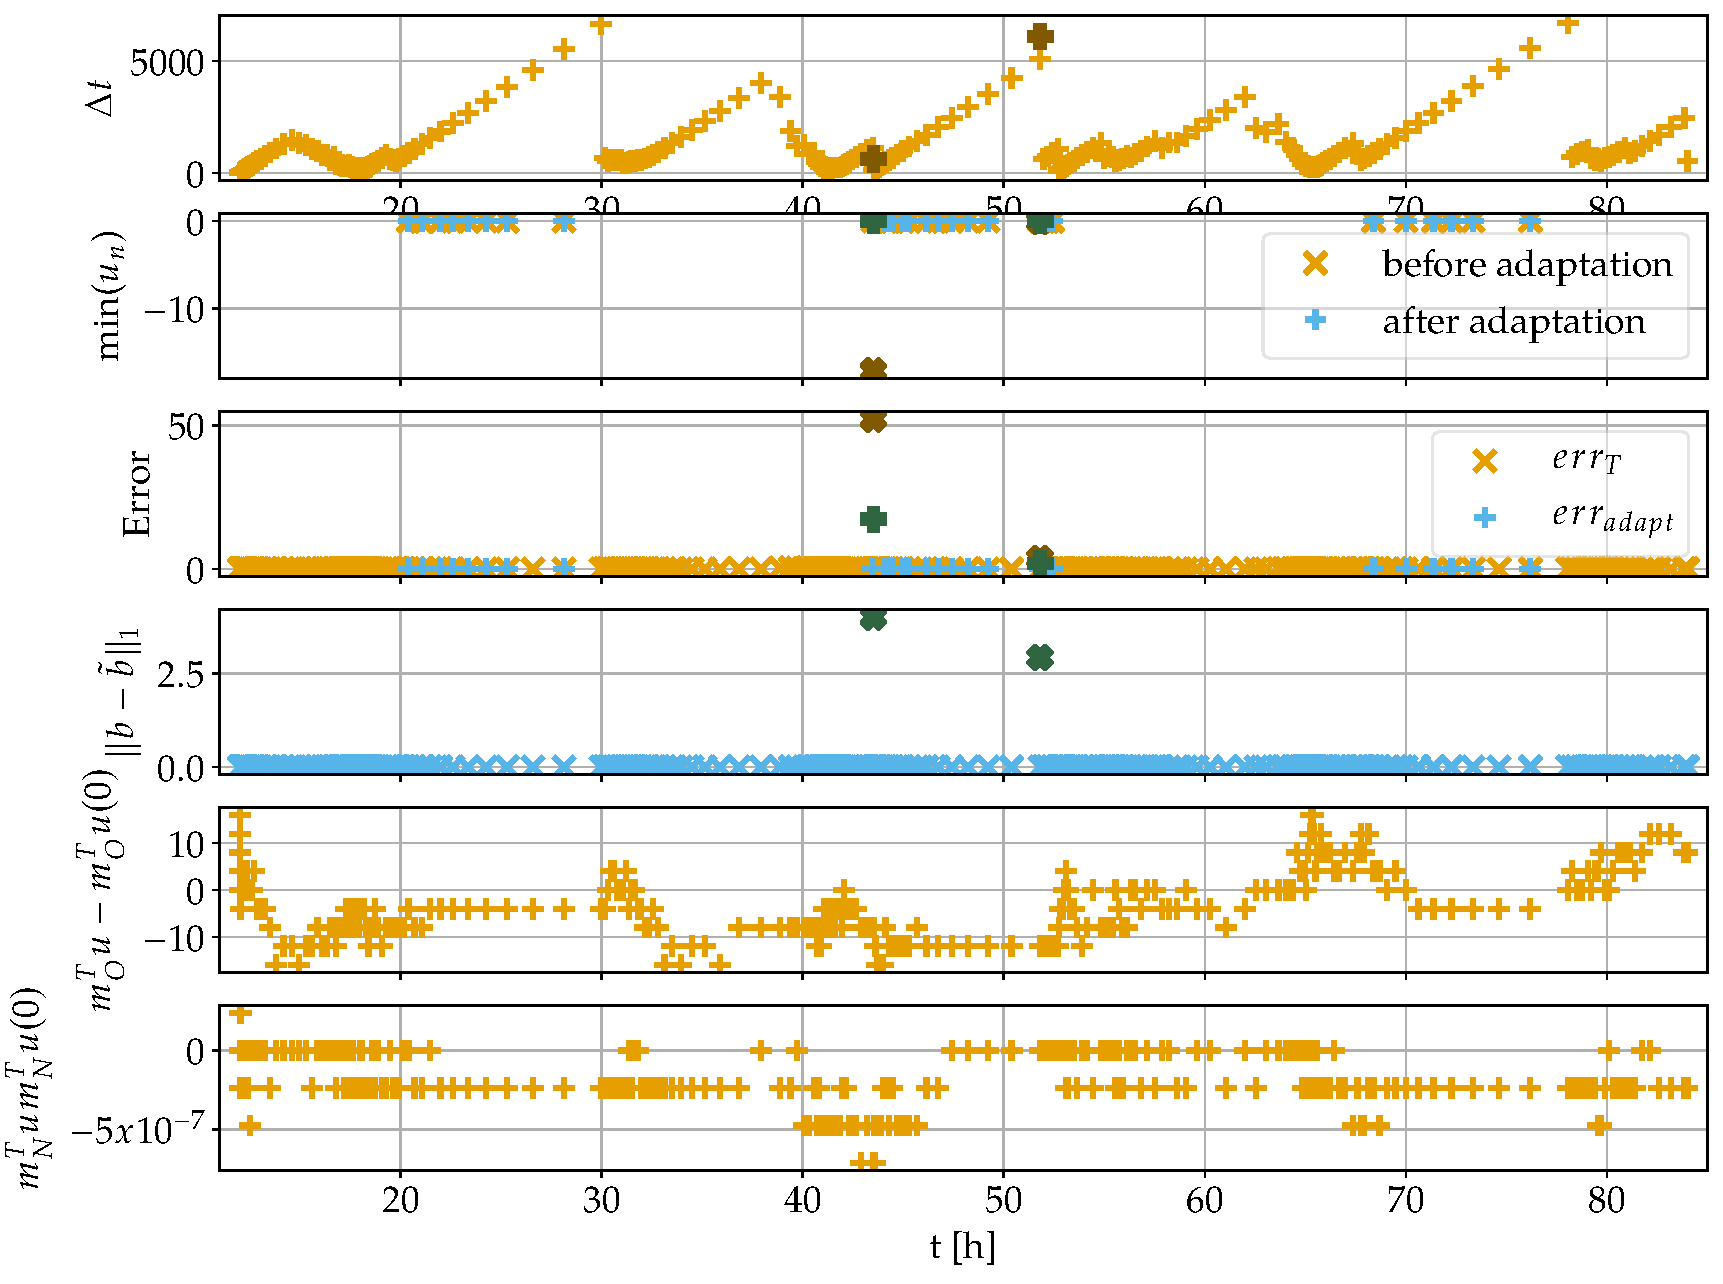
\includegraphics[width=0.85\textwidth]{plots/Stratospheric_stepsize,b.pdf}
\caption{Different statistics of computation of the stratospheric reaction.}
\label{fig:Stats_Strat}
\end{figure}


    